\chapter{Практические приложения}
\label{cha:applications}

В этой главе мы рассматриваем роль сингулярных элементов модулей аффинных алгебр Ли в приложениях к задачам конформной теории поля. Мы используем установленные в главах \ref{cha:affine-lie-algebras}, \ref{cha:BGG}, \ref{cha:splints} свойства для эффективных вычислений. 

\section{Роль сингулярных элементов coset-моделей в установлении соответствия между конформной теорией поля и критическим поведением в решеточных моделях}

% и  Эволюция Шрамма-Левнера и алгебраические свойства предельного перехода от решеточных моделей к конформной теории поля}
\label{sec:SLE}

Алгебраические методы в конформной теории поля позволяют получать явные уравнения на корреляционные функции (например, уравнения Книжника-Замолодчикова \eqref{eq:66} в ВЗНВ-моделях и их аналоги в coset-моделях \eqref{eq:101}). Во многих случаях эти уравнения можно решить аналитически либо численно и получить конкретные значения для физических величин, например, для критических индексов. Таким образом конформная теория поля является мощным инструментом для описания критического поведения в решеточных моделях. 

Однако соответствие между решеточными моделями и конформной теорией поля, описывающей их критическое поведение, не так легко установить. В случае простых моделей (Изинга, Поттса, Ашкина-Теллера и т.д.) и минимальных моделей конформной теории поля такое соответствие первоначально устанавливалось путем сравнения центральных зарядов и конформных размерностей. Но соответствие корреляторов нуждается в строгом доказательстве. Один из инструментов изучения решеточных моделей -- эволюция Шрамма-Левнера -- позволяет в некоторых случаях доказать такое соответствие (см. \cite{duminil2011conformal,chelkak2009universality,smirnov2007towards,smirnov2001critical,Cardy:2005kh,bauer2004conformal,bauer2004sle,bauer2004cfts,bauer2003sle,friedrich2003conformal,bauer2002sle}). Класс моделей конформной теории поля, для которых получены такие результаты, в основном ограничивается минимальными унитарными моделями. 

Введение дополнительного случайного блуждания на группе позволяет построить стохастический аналоги для ВЗНВ-моделей \cite{bettelheim2005stochastic,Rasmussen:2004xr,alekseev2010sle}. В данном разделе мы обсуждаем обобщение этой конструкции на случай coset-моделей.  В установлении соответствия между корреляторами в стохастических моделях и моделях конформной теории поля существенную роль играют сингулярные элементы, что связано со структурой модулей алгебры Вирасоро в ВЗНВ и coset-моделях (см. разделы \ref{sec:WZNW-models}\ref{sec:coset-models-cft}). К сожалению, пока не известно, пределами каких решеточных моделей могут являться такие стохастические конструкции.

Эволюция Шрамма-Левнера появляется как скейлинговый предел интерфейсов в решеточных моделях в критической точке. Критическое поведение этих моделей можно описывать при помощи минимальных моделей конформной теории поля. Оказывается, что некоторые корреляционные функции в моделях конформной теории поля являются мартингалами по отношению к эволюции Шрамма-Левнера. 
В этой главе мы обобщаем эволюцию Шрамма-Левнера с дополнительным броуновским движением на группе Ли  $G$ на случай фактор-пространства $G/A$. Замет мы изучаем, как связано такое описание критического поведения с coset-моделями конформной теории поля. В качестве критерия согласованности мы используем тот факт, что минимальные модели могут быть реализованы как coset-модели при некотором выборе групп $G, A$.

\subsection{Введение}
Эволюция Шрамма-Левнера -- это стохастический процесс, который предложил Oded Schramm  \cite{schramm2000scaling} для описания скейлингового предела критических интерфейсов в двумерных статистических решеточных моделях. Этот подход к критическим системам дал много строгих результатов в теории критического поведения (см. обзоры  \cite{rohde2005basic}, \cite{bauer20062d}, \cite{Cardy:2005kh}). В разделе \ref{sec:schr-loewn-evol} мы приводим необходимые определения.  

Вероятностная мера, порожденная эволюцией Шрамма-Левнера на случайных кривых, конформно-инвариантна. Так как конформная теория поля представляет собой другой метод для изучения двумерных критических систем, естественно изучать ее связь с эволюцией Шрамма-Левнера. Такая связь изучалась, например, в работах \cite{bauer2004conformal,bauer2004cfts,bauer2003sle,bauer2002sle} (и многих других), но в основном для минимальных унитарных моделей. 
Идея состоит в рассмотрении определенных наблюдаемых в области с разрезом. Эта конструкция обсуждается в разделе \ref{sec:corr-betw-sle}. 

Более общие модели конформной теории поля обладают дополнительными симметриями. Например,  в моделях Весса-Зумино-Новикова-Виттена возникают аффинные алгебры Ли.  Чтобы реализовать такие симметрии при изучении эволюции Шрамма-Левнера нужно ввести дополнительное случайное блуждание на группе Ли \cite{bettelheim2005stochastic}, \cite{Rasmussen:2004xr}. Такое случайное блуждание определяется в разделе \ref{sec:sle-wzw-models}. Соответствие между мартингалами эволюции Шрамма-Левнера и корреляционными функциями в моделях Весса-Зумино-Новикова-Виттена изучалось в работе \cite{alekseev2010sle}. Аналогичное обобщение на $\mathbb{Z}(N)$-парафермионную модель было предложено в статьях \cite{santachiara2008sle,picco2008numerical}. 

Основная задача данной главы состоит в обобщении эволюции Шрамма-Левнера с дополнительным случайным блужданием на группе Ли на случай фактор-пространства  $G/A$ и в изучении связи с coset-конструкцией конформной теории поля. В разделе \ref{sec:coset-models-sle} мы напоминаем некоторые детали coset-конструкции, вводим эволюцию Шрамма-Левнера на фактор-пространстве и связываем ее с конформной теорией поля. По аналогии со случаем моделей Весса-Зумино-Новикова-Виттена мы получаем систему алгебраических уравнений на оператор смены граничного условия из условия на мартингал. 
При помощи coset-конструкции можно реализовать минимальные и парафермионные модели конформной теории поля (см. \cite{difrancesco1997cft}), так что мы можем сравнить наши уравнения на оператор смены граничных условий с результатами работы \cite{santachiara2008sle}.

В разделе  \ref{sec:5-conclusion} мы обсуждаем возможность сравнения классификации операторов смены граничных условий, следующей из свойства мартингалов с общей классификацией операторов смены граничных условий в граничной конформной теории поля, связанной с D-бранными решениями \cite{fuchs2005geometry,fredenhagen2002d,elitzur2002d,Maldacena:2001ky,felder1999geometry,alekseev1999d}. 

\subsection{Эволюция Шрамма-Левнера}
\label{sec:schr-loewn-evol}
Рассмотрим модель Изинга на треугольной решетке в верхней полуплоскости (см. Рисунок \ref{fig:sle}). Наложим следующее граничное условие: потребуем, чтобы на одной половине границы все спины были направлены вверх, а на другой половине -- вниз. Тогда при любой конфигурации спинов на полуплоскости будет интерфейс, разделяющий два кластера и соединяющий точку ноль с бесконечностью (см. Рисунок \ref{fig:sle}).

\begin{figure}[h]
  \centering{
    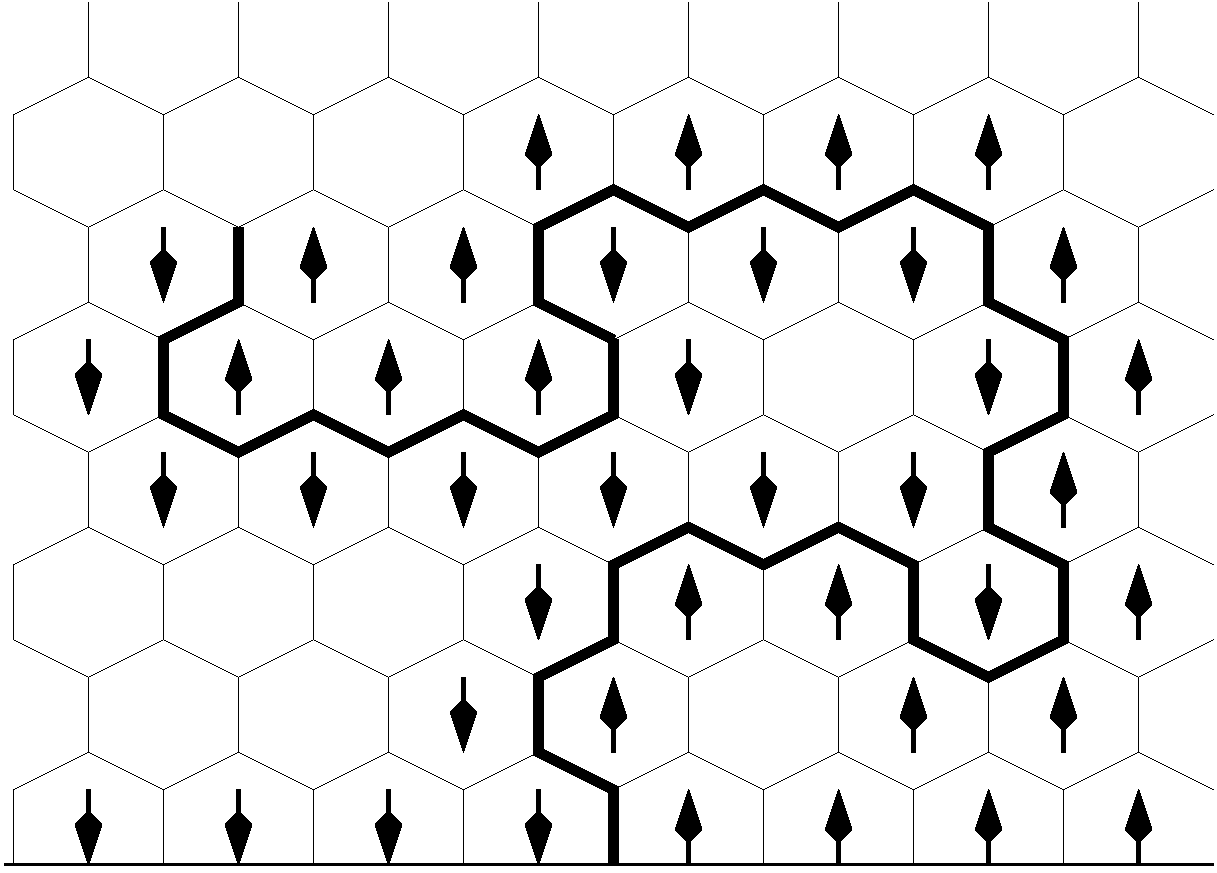
\includegraphics[height=50mm]{explore}
    \caption{Интерфейс в модели Изинга на треугольной решетке}}
  \label{fig:sle}
\end{figure}
Мы можем наложить условие существования части интерфейса конечной длины и рассмотреть конфигурации статистической модели, удовлетворяющие этому условию. Очевидно, такие конфигурации эквивалентны конфигурациям модели на области с разрезом вдоль интерфейса. 

Теперь рассмотрим непрерывный предел решеточной модели с (частью) интерфейса конечной длины. Интерфейсы в случайных конфигурациях модели сходятся к случайной кривой. Старая гипотеза \cite{Polyakov:1970xd} о конформной инвариантности в критической точке была недавно строго доказана для некоторых решеточных моделей (см. \cite{smirnov2007towards}, \cite{duminil2011conformal}). Мы предполагаем наличие конформной инвариантности в критической точке и рассматриваем верхнюю полуплоскость  $\mathbb{H}$ с разрезом вдоль критического интерфейса  $\gamma_{t}$. Такую область с разрезом мы обозначим через  $\mathbb{H}_{t}=\mathbb{H}\setminus \gamma_{t}$. Конформное отображение из $\mathbb{H}_{t}$ в $\mathbb{H}$ обозначим через $g_{t}:\mathbb{H}_{t}\to \mathbb{H}$ (см. Рисунок \ref{fig:sle2}).

\begin{figure}[h]
  \centering{
    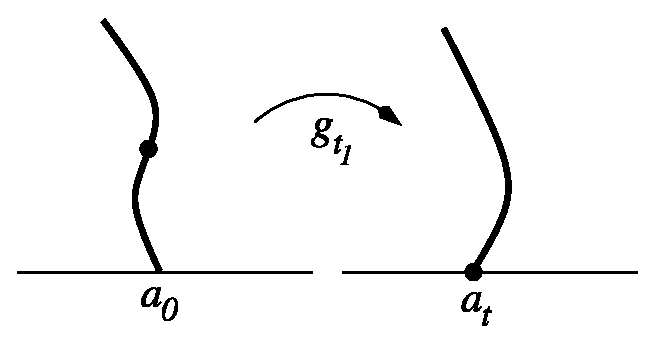
\includegraphics[width=60mm]{loewner}
    \caption{Конформное отображение $g_{t}(z):\mathbb{H}_{t}\to \mathbb{H}$.}}
  \label{fig:sle2}
\end{figure}

В статье \cite{schramm2000scaling} было показано, что  $g_{t}(z)$ удовлетворяет стохастическому дифференциальному уравнению
\begin{equation}
\label{eq:166}
  \frac{\partial g_t(z)}{\partial t} = \frac{ 2}{g_t(z)-\sqrt{\kappa}\xi_{t}} ,
\end{equation}
здесь $\xi_{t}$ -- Броуновское движение. Динамика конца  $z_{t}$ критической кривой $\gamma_{t}$ (конец следа эволюции Шрамма-Левнера) описывается уравнением $z_{t}=g_{t}^{-1}(\sqrt{\kappa}\xi_{t})$. 

Стохастический процесс, который удовлетворяет уравнению \eqref{eq:166} называется {\it эволюцией Шрамма-Левнера} на верхней полуплоскости $\mathbb{H}$. Для нас будет удобнее использовать отображение $w_{t} (z)=g_{t}(z)-\sqrt{\kappa}\xi_{t}$, так что уравнение \eqref{eq:166} переписывается в виде
\begin{equation}
  \label{eq:120}
       d w _{t}= \frac{2dt}{w_{t} }-\sqrt{\kappa}\xi_{t}  
\end{equation}
Эволюция Шрамма-Левнера порождает конформно-инвариантную вероятностную меру на кривых $\gamma_{t}$ в $\mathbb{H}$.

\subsection{Мартингалы эволюции Шрамма-Левнера и корреляционные функции в конформной теории поля}
\label{sec:corr-betw-sle}

Теперь рассмотрим наблюдаемые в присутствии следа эволюции Шрамма-Левнера. Математическое ожидание решеточной наблюдаемой $\mathcal{O}$ на верхней полуплоскости можно вычислить как сумму ожиданий этой наблюдаемой в присутствии (конечной части) траектории эволюции Шрамма-Левнера  $\gamma_{t}$ вплоть до некоторого времени $t$, умноженных на вероятность этой траектории:
\begin{equation*}
  \prec \mathcal{O} \succ_{\mathbb{H}}=\mathbb{E}\left[\prec\mathcal{O}\succ_{\gamma_{t}}\right]=\sum_{\gamma_{t}} P\left[C_{\gamma_{t}}\right] \prec \mathcal{O} \succ_{\gamma_{t}}
\end{equation*}
Решеточная наблюдаемая  $\prec \mathcal{O} \succ_{\mathbb{H}}$ не зависит от  $t$, следовательно $\prec\mathcal{O}\succ_{\gamma_{t}}$ -- мартингал.

В непрерывном пределе решеточные наблюдаемые сходятся к корреляционным функциям в конформной теории поля \cite{bauer2003sle,bauer2003conformal,bauer2002sle}. Мы должны учесть изменение граничных условий на конце следа эволюции Шрамма-Левнера и на бесконечности, так что соотношение имеет вид:
\begin{equation}
  \prec \mathcal{O} \succ_{\mathbb{H}_{t}}\to \mathcal{F}(\left\{z_{i}\right\})_{\mathbb{H}_{t}}=
  \frac{\left< \mathcal{O}(\{z_{i}\})\phi(z_{t})\phi^{\dagger}(\infty)\right>_{\mathbb{H}_{t}}}{\left<\phi(z_{t})\phi^{\dagger}(\infty)\right>_{\mathbb{H}_{t}}}
%% =
%%   \frac{\left<^{g_{t}}
%% \mathcal{O}\phi(\xi_{t})\phi^{\dagger}(\infty)\right>_{\mathbb{H}}}{\left<\phi(\xi_{t})\phi^{\dagger}(\infty)\right>_{\mathbb{H}}}
\label{eq:162}
\end{equation}

%% Here $\phi(z_{t})$ is a primary field corresponding to boundary condition changing operator.
%% We've used the conformal map $g_{t}$ to get the expression on the whole plane in equation \eqref{eq:162}.
Мы рассматриваем теорию с границей, так что мы должны использовать модели граничной конформной теории поля и накладывать соответствующие граничные условия \cite{cardy1984conformal,cardy1989boundary,cardy1991bulk}. В случае верхней полуплоскости корреляционные функции в граничной конформной теории поля могут быть переписаны как корреляционные функции для теории на всей плоскости, но с удвоенным числом полей.

% Here we are interested mainly in properties of boundary condition changing operator $\phi$. 

Мы предполагаем, что $\mathcal{F}$ содержит некоторый набор примарных полей  $\varphi_{\lambda_{i}}$ с конформными весами $h_{\lambda_{i}}$. Так как мы рассматриваем граничную конформную теорию поля, мы должны добавить объемные поля в сопряженных точках  $\bar z_{i}$. Для дальнейшего использования в моделях Весса-Зумино-Новикова-Виттена мы обозначим конформные веса этих сопряженных полей через $h_{\lambda_{i}^{*}}$. Кроме того, у нас есть операторы смены граничного условия   $\phi$ на конце следа эволюции Шрамма-Левнера и на бесконечности. Воспользуемся конформным отображением   $w(z):\mathbb{H}\setminus\gamma_{t}\to \mathbb{H}$, чтобы переписать выражение \eqref{eq:162} на верхней полуплоскости без разреза:
\begin{equation}
  \mathcal{F}(\left\{z_{i}\right\})_{\mathbb{H}_{t}}=\prod \left(\frac{\partial w(z_{i})}{\partial z_{i}}\right)^{h_{\lambda_i}} 
  \prod \left(\frac{\partial \bar w(\bar z_{i})}{\partial \bar z_{i}}\right)^{h_{\lambda^{*}_i}}
  \mathcal{F}(\left\{w_{i}, \bar w_{i}\right\})_{\mathbb{H}}
  \label{eq:69}
\end{equation}

Теперь нам нужно рассмотреть, как преобразуется конец следа эволюции Шрамма-Левнера  $\gamma_{t}$ при переходе от времени $t$ к $t+ dt$. Первый множитель в правой части уравнения  (\ref{eq:69}) дает нам
\begin{equation*}
  -\frac{2h_{\lambda_{i}}}{w_{i}^{2}}\left(\frac{\partial w_{i}}{\partial z_{i}}\right)^{h_{\lambda_{i}}}.
\end{equation*}
Для преобразования примарных полей  $\varphi_{\lambda_{i}}$ имеет место равенство
\begin{equation}
\label{eq:70}
  d\varphi_{\lambda_{i}}(w_{i}) = \mathcal{G}_{i}\varphi_{\lambda_{i}}(w_{i})=\left(\frac{2dt}{w_{i}}-\sqrt{\kappa} d\xi_{t}\right) \partial_{w_{i}}\varphi_{\lambda_{i}}(w_{i}) 
\end{equation}
Мы обозначим генератор этого преобразования через  $\mathcal{G}_{i}$.

Так как $ \prec\mathcal{O}\succ_{\gamma_{t}}$ --  мартингал, математическое ожидание его приращения при эволюции от  $t$ к $t+dt$ равняется нулю
\begin{equation}
  \mathbb{E}\left[\prec\mathcal{O}\succ_{\gamma_{t}}\right]=    \mathbb{E}\left[\prec\mathcal{O}\succ_{\gamma_{t+dt}}\right], \quad d\mathbb{E}\left[ \prec\mathcal{O}\succ_{\gamma_{t}}\right]=0
\label{eq:163}
\end{equation}
Используем исчисление Ито и получим выражение для дифференциала $\mathcal{F}$:
\begin{equation}
d \mathcal{F}_{\mathbb{H}_{t}}= \left(\prod_{i=1}^{2N}\left(\frac{\partial w_{i}}{\partial z_{i}}\right)^{h_{i}}\right)\left(-\sum_{i=1}^{2N}\frac{2h_{i}dt}{w_{i}^{2}}+\left[\sum_{i=1}^{2N}\mathcal{G}_{i}+\frac{1}{2}
      \sum_{i,j}\mathcal{G}_{i}\mathcal{G}_{j}\right]\right)\mathcal{F}_{\mathbb{H}}=0
\label{eq:150}
\end{equation}
Подставим формулу \eqref{eq:70} и получим уравнение
\begin{equation}
  \left( \sum_{i}\left[-\frac{2h_{i}}{w_{i}^{2}} +\frac{2}{w_{i}}\partial_{w_{i}}\right]+\frac{\kappa}{2}\sum_{i,j}\partial_{w_{i}} \partial_{w_{j}}\right)\mathcal{F}(\left\{z_{i}\right\})=0
\label{eq:165}
\end{equation}

Для корреляционных функций вторичных полей  $L_{-n}\phi$ имеет место уравнение
\begin{equation}
\left< (L_{-n}\phi)(z) \varphi_{1}\dots \varphi_{N}\right>=\mathcal{L}_{-n}\left<\phi\varphi_{1}\dots\varphi_{N}\right>,
\end{equation}
где $n\geq 1$ и
\begin{equation*}
  \mathcal{L}_{-n}=\sum_{i=1}^{N} \left(\frac{(n-1)h_{i}}{(w_{i}-z)^{n}} -\frac{1}{(w_{i}-z)^{n-1}}\partial_{w_{i}}\right)
\end{equation*}
(См. \cite{difrancesco1997cft}). То есть мы можем переписать дифференциальное уравнение \eqref{eq:165} как алгебраическое уравнение на поле $\phi$, соответствующее оператору смены граничных условий:
\begin{equation}
  \label{eq:168}
   \left<\left([L_{-2}-\frac{\kappa}{2}L_{-1}^{2}]\phi\right)(0)\; \varphi_{\lambda_{1}}\dots \varphi_{\lambda_{{2N}}}\right>=0.
\end{equation}
В случае минимальных моделей набор примарных полей конечен и все состояния можно получить через соответствие между полями и состояниями
\cite{belavin1984ics}, \cite{difrancesco1997cft}. 
Равенство \eqref{eq:168} верно для произвольной наблюдаемой $\mathcal{O}$ и для произвольных примарных поле $\varphi_{\lambda_{i}}$, так что $\psi=[L_{-2}-\frac{\kappa}{2}L_{-1}^{2}]\phi$ -- нулевое поле уровня два и $\psi(0)\left|0\right>$ -- нулевое состояние уровня два. В минимальных унитарных моделях существует только два примарных поля, порождающих модули Верма алгебры Вирасоро с нулевыми состояниями на уровне два. Это поля $\phi_{1,2}$ и $\phi_{2,1}$, так что $\phi\sim \phi_{1,2} \;\text{or}\; \phi_{2,1}$. 

\subsection{Модели Весса-Зумино-Новикова-Виттена и эволюция Шрамма-Левнера}
\label{sec:sle-wzw-models}
Чтобы обобщить анализ предыдущего раздела  \ref{sec:corr-betw-sle} на не-минимальные модели мы должны принять во внимание дополнительные симметрии. Модели Весса-Зумино-Новикова-Виттена обладают симметрией Каца-Муди в дополнение к конформной инвариантности, приводящей к появлению алгебры Вирасоро. Сначала мы напомним свойства ВЗНВ-моделей \cite{difrancesco1997cft}, которые нужны для изучения мартингалов эволюции Шрамма-Левнера.

Действие модели Весса-Зумино-Новикова-Виттена записывается в терминах отображения $g:\mathbb{C}\cup \{\infty\}\sim S^{2}\to G$ из комплексной плоскости с бесконечностью (сферы Римана) в некоторую (простую) группу Ли $G$:
\begin{multline}
  S=-\frac{k}{8\pi}\int d^2x\; \mathcal{K} (g^{-1}\partial^{\mu}g, g^{-1} \partial_{\mu}g)  
  - \frac{k }{24\pi^{2}} \int_{B}\epsilon_{ijk} \mathcal{K}\left(
    \tilde g^{-1}\frac{\partial \tilde g}{\partial y^i},\left[
      \tilde g^{-1}\frac{\partial \tilde g}{\partial y^j}
      \tilde g^{-1}\frac{\partial \tilde g}{\partial y^k}\right]\right) d^3y
\end{multline}
Здесь $\mathcal{K}$ -- форма Киллинга на алгебре Ли  $\gf$ группы Ли $G$. Первый член -- это просто нелинейная сигма-модель, а второй записывается при помощи продолжения $\tilde{g}$ с два-сферы $S^{2}$ на трехмерное многообразие $B$, границей которого является два-сфера. Так как это продолжение не единственно, а экспонента действия должна быть определена однозначно, константа  $k$ должна быть целочисленной.

Сохраняющиеся токи в этой модели даются выражениями:
  \begin{eqnarray}
    J(z)= -k \partial_zg g^{-1}
    \bar J(\bar z)=k g^{-1}\partial_{\bar z}g
  \end{eqnarray}

Модель обладает калибровочной инвариантностью по отношению к преобразованиям
  $g(z,\bar z)\to \Omega(z)g(z,\bar z)\bar \Omega^{-1}(\bar z)$, 
здесь $\Omega,\;\bar \Omega \in G$ независимы. Из рассмотрения инфинитезимальных калибровочных преобразований  $\Omega=1+\omega$ получаем тождества Уорда
  \begin{equation}
    \label{eq:139}
    \delta_{\omega,\bar \omega}\left< X \right>=-\frac{1}{2\pi i}\oint dz \sum\omega^a \left< J^a X\right>+
    \frac{1}{2\pi i} \oint d\bar z \sum \bar \omega^a \left< \bar J^a X\right>,
  \end{equation}
из которых следует операторное разложение для токов:
 \begin{equation}
   \label{eq:128}
   J^{a}(z)J^{b}(w)\sim \frac{k\delta_{ab}}{(z-w)^{2}}+\sum_{c}i f_{abc}\frac{J^{c}}{z-w},
 \end{equation}
здесь $f_{abc}$ -- структурные константы алгебры Ли $\gf$.
 
Разложим токи на моды $J^a(z)=\sum\limits_{n\in \mathbb Z}z^{n-1}J^a_n $, воспользуемся операторным разложением \eqref{eq:128} и получим коммутационные соотношения аффинной алгебры Ли $\gfh$:
\begin{equation*}
 \left[J^a_n,J^b_m\right]=\sum_c i f^{abc}J^c_{n+m}+kn\delta^{ab}\delta_{n+m,0}.  
\end{equation*}

Конформная инвариантность в этой модели следует из конструкции Сугавары, которая представляет собой способ вложения алгебры Вирасоро в универсальную обертывающую алгебры аффинной алгебры Ли $\gfh$ ($Vir\subset U(\gfh)$):
\begin{equation}
  \label{eq:134}
  L_n=\frac{1}{2(k+h^{\vee})}\left(\sum\limits_a\sum\limits_{m\leq -1}J^a_m J^a_{n-m}+\sum_{m\geq 0} J^{a}_{n-m}J^{a}_{m}\right), 
\end{equation}
где $h^{\vee}$ -- дуальное число Кокстера алгебры Ли $\gf$. 
Полная киральная алгебра модели представляет собой полупрямое произведение аффинной алгебры и алгебры Вирасоро $\gfh \ltimes Vir$ с коммутационными соотношениями
  \begin{equation}
    \label{eq:141}
    \begin{aligned}
      \left[J^a_n,J^b_m\right]=\sum_c i f^{abc}J^c_{n+m}+kn\delta^{ab}\delta_{n+m,0} \\
      \left[L_n,L_m\right]=(n-m)L_{n+m}+\frac{c}{12}(n^3-n)\delta_{n+m,0}\\
      \left[L_n,J^a_m\right]=-mJ^a_{n+m}
    \end{aligned}
  \end{equation}
Здесь центральный заряд  $c$ алгебры Вирасоро дается выражением
\begin{equation}
  \label{eq:164}
  c=\frac{k\;\mathrm{dim}\gf}{k+h^{\vee}}
\end{equation}
В модели существует бесконечное число полей, примарных по отношению к действию алгебры Вирасоро, но они организованы в модули старшего веса аффинной алгебры Ли $\gfh$. Примарные поля полной киральной алгебры  $\phi_{\lambda}$ нумеруются старшими весами  $\gfh$-модулей. Покажем, как генераторы алгебры Вирасоро и аффинной алгебры Ли действуют на примарные поля:
  \begin{equation*}
    \begin{aligned}
      & J_0^a\left|\phi_{\lambda}\right>=-t^a_{\lambda}\left|\phi_{\lambda}\right>  \quad    J^a_n\left|\phi_{\lambda}\right>=0 \quad \text{для}\; n>0 \\
      & L_0\left|\phi_{\lambda}\right>=\frac{1}{2(k+h^{\vee})}\sum_aJ^a_0J^a_0\left|\phi_{\lambda}\right>=\frac{(\lambda,\lambda+2\rho)}{2(k+h^{\vee})}\left|\phi_{\lambda}\right>=h_{\lambda} \left|\phi_{\lambda}\right>,
    \end{aligned}
  \end{equation*}
где $\rho$ -- вектор Вейля алгебры $\gf$. 

Теперь рассмотрим эволюцию Шрамма-Левнера в ВЗНВ-моделях. 
Подобно минимальным моделям мы рассматриваем наблюдаемые
\begin{equation*}
  \mathcal{F}(\left\{z_{i}\right\})_{\mathbb{H}_{t}}=
  \frac{\left<\phi_{\Lambda}(z_{t}) \phi_{\lambda_1}(z_{1}) \dots \phi_{\lambda_n}(z_{n}) \phi_{\lambda^{*}_1}(\bar z_{1}) \dots \phi_{\lambda^{*}_n}(\bar z_{n})
      \phi_{\Lambda^{*}}(\infty)\right>}{\left<\phi_{\Lambda}(z_{t})\phi_{\Lambda^{*}}(\infty)\right>}
\end{equation*}
Мы опять используем конформное отображение  $w(z):\mathbb{H}\setminus\gamma_{t}\to \mathbb{H}$ чтобы переписать формулу для наблюдаемых на всей верхней полуплоскости.
\begin{equation}
  \mathcal{F}(\left\{z_{i}\right\})_{\mathbb{H}_{t}}=\prod \left(\frac{\partial w(z_{i})}{\partial z_{i}}\right)^{h_{\lambda_i}} 
  \prod \left(\frac{\partial \bar w(\bar z_{i})}{\partial \bar z_{i}}\right)^{h_{\lambda^{*}_i}}
  \mathcal{F}(\left\{w_{i}, \bar w_{i}\right\})_{\mathbb{H}}
  \label{eq:177}
\end{equation}

В результате эволюции от $t$ к $t+dt$ первый множитель дает нам $-\frac{2h_{\lambda_{i}}}{w_{i}^{2}}\left(\frac{\partial w_{i}}{\partial z_{i}}\right)^{h_{\lambda_{i}}}$.

При рассмотрении полей нам нужно добавить случайное калибровочное преобразование  (случайное блуждание в $G$) к стохастическому процессу \cite{bettelheim2005stochastic}, \cite{alekseev2010sle}. 
Для полей мы имеем
\begin{equation*}
  d\phi_{\lambda_{i}}(w_{i}) = \mathcal{G}_{i}\phi_{\lambda_{i}}(w_{i}),
\end{equation*}
так что в генераторе преобразования поля появляется дополнительный член
\begin{equation}
  \mathcal{G}_{i}=\left(\frac{2dt}{w_{i}}-\sqrt{\kappa} d\xi_{t}\right) \partial_{w_{i}}+\frac{\sqrt{\tau}}{w_{i}}\sum_{a=1}^{\mathrm{dim} \gf}\left(d \theta ^{a} t^{a}_{i}\right)
\label{eq:159}
\end{equation}
Здесь  $d\theta^{a}$ -- генераторы  $\mathrm{dim}\gf$--мерного Броуновского движения, с $\mathbb{E}[d\theta^{a}d\theta^{b}]=\delta_{ab}dt$. Мы предполагаем, что $t^{a}$ -- это базис в $\gf$, ортогональный по отношению к форме Киллинга $\mathcal{K}$, $\mathcal{K}(t^{a},t^{b})=\delta_{ab}$.

Воспользуемся формулой \eqref{eq:150} и получим следующее уравнение из условий для мартингала:
\begin{equation}
  \left(-2 \mathcal{L}_{-2}+\frac{1}{2}\kappa \mathcal{L}_{-1}^{2}+\frac{1}{2}\tau\sum_{a} \mathcal{J}^{a}_{-1} \mathcal{J}^{a}_{-1}\right)        \mathcal{F}(\left\{w_{i}, \bar w_{i}\right\})_{\mathbb{H}}=0,
  \label{eq:167}
\end{equation}
где
\begin{equation*}
  \mathcal{L}_{-n}=\sum_{i}\left(\frac{(n-1)h_{\lambda_{i}}}{(w_{i}-z)^{n}}-\frac{1}{(w_{i}-z)^{n-1}}\partial_{w_{i}}\right);\quad \mathcal{J}^{a}_{{-n}}=-\sum_{i}\frac{t^{a}_{i}}{(w_{i}-z)^{n}}
\end{equation*}
Мы снова перепишем уравнение в виде алгебраического соотношения на поле, соответствующее оператору смены граничного условия. Теперь
\begin{equation}
  \left| \psi\right>=\left(-2 L_{-2}+\frac{1}{2}\kappa L_{-1}^{2}+\frac{1}{2}\tau\sum_{a} J^{a}_{-1} J^{a}_{-1}\right) \left|\phi_{\Lambda}\right>    
  \label{eq:16}
\end{equation}
является нулевым состоянием уровня два и если на него подействовать повышающими операторами, мы должны получить ноль.
\begin{eqnarray}
  J^{a}_{1} \left|\psi\right>=0\\
  J^{a}_{2}\left|\psi\right>=0\\
  L_{2}\left|\psi\right>=0\\
  L_{1}\left|\psi\right>=0
\end{eqnarray}
Эти уравнения можно переписать как алгебраические соотношения, связывающие параметры случайного блуждания $\kappa, \tau$ с уровнем  $k$ представления аффинной алгебры Ли, если воспользоваться коммутационными соотношениями  \eqref{eq:141}. Строгий анализ полученных алгебраических соотношений проведен в работе \cite{alekseev2010sle}.

\subsection{Coset-модели и эволюция Шрамма-Левнера}
\label{sec:coset-models-sle}
Теперь мы обобщим анализ соответствия между эволюцией Шрамма-Левнера и конформной теорией поля на случай coset-моделей \cite{Goddard198588}. Такие модели задаются алгеброй Ли $\gf$ и ее подалгеброй $\af$. Обозначим через $J_{n}^{a}$ генераторы аффинной алгебры Ли $\gfh$, а через $\tilde{J}_{n}^{b}$ -- генераторы $\afh$, так что $\tilde{J}^{b}_{n}=\sum_{a} m_{a}^{b} J^{a}_{n}$. Генераторы алгебры Вирасоро в coset-моделях даются разностями выражений Сугавары для ВЗНВ-моделей, соответствующих алгебрам  $\gf$ и $\af$:
\begin{equation*}
  L_{n}=L_{n}^{\gf}-L_{n}^{\af}
\end{equation*}
Коммутационные соотношения между генераторам алгебры Вирасоро и генераторами подалгебры  $\afh$ тривиальны
\begin{equation}
  \label{eq:156}
  \left[L_{n},\tilde{J}^{b}_{m}\right]=0
\end{equation}

Поля нумеруются парами весов  $(\mu,\nu)$, где $\mu$ -- вес  $\gfh$, а $\nu$ -- вес $\afh$, соответственно. Но появляются правила отбора, так как функции ветвления для некоторых пар весов  $(\mu,\nu)$ исчезают. Кроме того, имеется избыточность, так как функции ветвления для различных пар $(\mu,\nu)$ могут совпадать \cite{fuchs1996resolution,schellekens1990field}.

Итак, примарные поля нумеруются парами весов  $(\mu,\nu)\in \hf_{\gfh}\oplus \hf_{\afh}$ алгебры $\gfh$ и подалгебры $\afh$, такими, что соответствующие функции ветвления $b^{\mu}_{\nu}(q)\neq 0$. Некоторые пары эквивалентны. Эта эквивалентность дается действием так называемых ``простых токов'' $(J,\tilde{J})$, которые являются элементами группы внешних автоморфизмов  $\mathcal{O}(\gfh)\times \mathcal{O}(\afh)\approx B(G)\times B(A)$ алгебры $\gfh\times\afh$, где $B(G)$ -- это центр группы Ли $G$. Мы можем думать о простых токах как о примарных полях, тогда их действие на поля теории дается слиянием \cite{difrancesco1997cft}. Таким образом, примарные поля coset-моделей нумеруются классами эквивалентности пар весов  $(\mu,\nu)\sim (J*\mu,\tilde{J}*\nu)$, где $(J,\tilde J)$ такие, что  конформные веса компонент равны:  $h_{J}-h_{\tilde{J}}=0$. 

Конформный вес примарного поля в coset-модели равен
\begin{multline}
  L_0\left|\phi_{(\mu,\nu)}\right>=\left(\frac{1}{2(k+h^{\vee})}\sum_aJ^a_0J^a_0-\frac{1}{2(k+h_{\af}^{\vee})}\sum_b \tilde{J}^b_0 \tilde{J}^b_0 \right)
  \left|\phi_{(\mu,\nu)}\right>=\\
  \left(\frac{(\mu,\mu+2\rho)}{2(k+h^{\vee})}-\frac{(\nu,\nu+2\rho_{\af})}{2(k+h^{\vee})}\right)\left|\phi_{(\mu,\nu)}\right>
\end{multline}
Можно получить аналог уравнений Книжника-Замолодчикова для coset-моделей \cite{kogan1997knizhnik}:
\begin{equation}
  \left\{\frac{1}{2}\partial_{i} + \sum_{i\neq j}^{N}\left(\frac{t^{a}_{i}t^{a}_{j}}{k+h^{\vee}}-\frac{\tilde t^{b}_{i}\tilde t^{b}_{j}}{k+h^{\vee}_{\af}}\right)\frac{1}{z_{i}-z_{j}}\right\} \left<\phi_{1}(z_{1})\dots \phi_{N}(z_{N})\right>=0
  \label{eq:144}
\end{equation}

Как мы упоминали в главе \ref{cha:CFT}, $G/A$-coset модель конформной теории поля может быть реализована как ВЗНВ-модель (с калибровочной группой $G$), взаимодействующая с чисто калибровочными полями, с калибровочной группой $A\subset G$ \cite{gawdzki1988g,figueroa89equivalence}. Действие записывается через поля $\gamma:\mathbb{C}\to G$ and $\alpha,\bar\alpha:\mathbb{C}\to A$ следующим образом:
\begin{multline}
  \label{eq:24}
      S_{G/A}(\gamma, \alpha)=-\frac{k}{8\pi}\int_{S^2} d^2x\; {\cal K} (\gamma^{-1}\partial^{\mu}\gamma,\gamma^{-1}\partial_{\mu}\gamma)-\\
 - \frac{k }{24\pi} \int_{B}\epsilon_{ijk} {\cal K}\left(
    \tilde \gamma^{-1}\frac{\partial \tilde \gamma}{\partial y^i},
      \left[\tilde \gamma^{-1}\frac{\partial \tilde \gamma}{\partial y^j}
      \tilde \gamma^{-1}\frac{\partial \tilde \gamma}{\partial y^k}\right]\right) d^3y+\\
+
      \frac{k}{4\pi}\int_{S^2} d^{2}z \left(\mathcal{K}(\alpha, \gamma^{-1}\bar \partial \gamma)-\mathcal{K}(\bar \alpha, (\partial \gamma ) \gamma^{-1})\right.\\
      \left.+\mathcal{K}(\alpha,\gamma^{-1}\bar \alpha \gamma)-\mathcal{K}(\alpha,\bar \alpha)\right).
\end{multline}
Здесь через  $\mathcal{K}$ обозначена форма Киллинга в алгебре Ли $\gf$, соответствующей группе Ли $G$.

Если мы фиксируем  $A$-калибровку, у нас останется  $G/A$ калибровочная инвариантность. Значит мы должны добавить случайные калибровочные преобразования к эволюции Шрамма-Левнера, аналогично случаю ВЗНВ-моделей из предыдущего раздела (См. также \cite{bettelheim2005stochastic}).  Обозначим через $t^{a}_{i}$ ($\tilde{t}^{b}_{i}$) генераторы представления алгебры $\gf$ (соответственно, представления $\af$), соответствующего примарному полю $\phi_{i}$.

Рассмотрим эволюцию следа SLE $\gamma_{t}$ с момента   $t$ до $t+ dt$.  Первый сомножитель в правой части уравнения (\ref{eq:177}) дает нам
\begin{equation*}
  -\frac{2h_{i}}{w_{i}^{2}}\left(\frac{\partial w_{i}}{\partial z_{i}}\right)^{h_{i}}.
\end{equation*}
We denote by $\mathcal{G}_{i}$ the generator of infinitesimal transformation of primary field $\phi_{i}$:$d\phi_{i}(w_{i}) = \mathcal{G}_{i}\phi_{i}(w_{i})$. We normalize additional $\left(\dim\gf\right)$-dimensional Brownian motion as $\mathbb  {E}\left[d\theta^{a}\; d\theta^{b}\right]=\mathcal{K}(t^{a},t^{b})dt$. The generator of field transformation is equal to
\begin{equation}
  \mathcal{G}_{i}=\left(\frac{2dt}{w_{i}}-\sqrt{\kappa} d\xi_{t}\right) \partial_{w_{i}}+\frac{\sqrt{\tau}}{w_{i}}\left(\sum_{a:\mathcal{K}(t^{a},\tilde{t}^{b})=0}\left(d \theta ^{a} t^{a}_{i}\right)\right).
\label{eq:3}
\end{equation}
So we have fixed $A$-gauge by allowing random walk only in direction orthogonal to subalgebra $\af$. 

 Ito formula  gives us an expression for the differential of $\mathcal{F}$ which should be zero due to martingale condition:
\begin{multline}
d \mathcal{F}_{\mathbb{H}_{t}}=\\ \left(\prod_{i=1}^{2N}\left(\frac{\partial w_{i}}{\partial z_{i}}\right)^{h_{i}}\right)
\left(-\sum_{i=1}^{2N}\frac{2h_{i}dt}{w_{i}^{2}}+\left[\sum_{i=1}^{2N}\mathcal{G}_{i}+\frac{1}{2}
      \sum_{i,j}\mathcal{G}_{i}\mathcal{G}_{j}\right]\right)\mathcal{F}_{\mathbb{H}}\\=0
\label{eq:8}
\end{multline}
Substituting  definition \eqref{eq:3} we get 
\begin{equation}
  \left(-2 \mathcal{L}_{-2}+\frac{1}{2}\kappa \mathcal{L}_{-1}^{2}+\frac{\tau}{2}\left( \sum_{a} \mathcal{J}^{a}_{-1} \mathcal{J}^{a}_{-1}-
      \sum_{b}\tilde{\mathcal{J}}^{b}_{-1} \tilde{\mathcal{J}}^{b}_{-1}\right)\right)        \mathcal{F}_{\mathbb{H}}=0,
  \label{eq:4}
\end{equation}
with
\begin{eqnarray*}
  \mathcal{L}_{-n}=\sum_{i}\left(\frac{(n-1)h_{i}}{(w_{i}-z)^{n}}-\frac{\partial_{w_{i}}}{(w_{i}-z)^{n-1}}\right),\\ \mathcal{J}^{a}_{{-n}}=-\sum_{i}\frac{t^{a}_{i}}{(w_{i}-z)^{n}};\; \tilde{\mathcal{J}}^{b}_{{-n}}=-\sum_{i}\frac{\tilde{t}^{b}_{i}}{(w_{i}-z)^{n}}.
\end{eqnarray*}
This equation is equivalent to the following algebraic condition on the boundary state $\varphi(0)\left|0\right>$:
\begin{multline}
  \label{eq:7}
  \left<0\left|\varphi(\infty)\phi_{1}(w_{1})\dots\phi_{2N}(w_{2N})\right.\right.\\
  \left(-2L_{-2}+\frac{1}{2}\kappa L_{-1}^{2}+\frac{1}{2}\tau \left(\sum_{a=1}^{\dim\gf}J^{a}_{-1}J^{a}_{-1}-\sum_{b=1}^{\dim\af}\tilde{J}^{b}_{-1}\tilde{J}^{b}_{-1}\right)\right)\\
\left.\varphi(0)|0\right>=0.
\end{multline}
Since the set $\{\phi_{i}\}$ consists of arbitrary primary fields we conclude that 
\begin{multline}
|\psi>=\left(-2L_{-2}+\frac{1}{2}\kappa L_{-1}^{2}+\frac{1}{2}\tau \left(\sum_{a=1}^{\dim\gf}J^{a}_{-1}J^{a}_{-1}-\sum_{b=1}^{\dim\af}\tilde{J}^{b}_{-1}\tilde{J}^{b}_{-1}\right)\right)\\
\cdot\varphi(0)|0>
\end{multline}
is a null-state. Now we act on $\psi$ by raising operators to get equations on $\kappa,\tau$. Since in a coset theory commutation relations of full chiral algebra are
\begin{equation}
  \label{eq:18}
\begin{array}{ll}
  L_{n}= L_{n}^{\gf}-L_{n}^{\af}, &\\
  \left[L_{n}^{\gf},J^{a}_{m}\right]= -m J^{a}_{n+m},&\\
  \left[L_{n}^{\gf},\tilde{J}^{b}_{m}\right]=-m\tilde{J}^{b}_{n+m},&\\
  \left[L_{n}^{\gf},L_{m}\right]=[L_{n}^{\gf},L_{m}^{\gf}]-[L_{n}^{\gf},L_{m}^{\af}]=&\\
  \quad =(n-m)L_{m+n}+\frac{c}{12}(n^{3}-n)\delta_{m+n,0},&
\end{array}
\end{equation}
 it is more convenient to act with $L_{2}^{\gf}$ and $\left(L_{1}^{\gf}\right)^{2}$. 
 Applying $L_{2}^{\gf}$ we get
\begin{equation*}
  L_{2}^{\gf}\psi= \left(-8 L_{0}-c+ 3 \kappa L_{0}+\frac{1}{2}\tau (k \dim\gf-x_{e}k\dim\af)\right) \varphi_{(\mu,\nu)}=0
\end{equation*}
We use $L_{0} \varphi_{(\mu,\nu)}=h_{(\mu,\nu)} \varphi_{(\mu,\nu)}$, with the conformal weight  $h_{(\mu,\nu)}= \left(\frac{(\mu,\mu+2\rho)}{2(k+h^{\vee}_{\gf})}-\frac{(\nu,\nu+2\rho_{\af})}{2(k x_{e}+h^{\vee}_{\af})}\right)$ and the central charge $c=\frac{k\dim \gf}{k+h^{\vee}_{\gf}}-\frac{x_{e}k\dim \af}{x_{e} k+h^{\vee}_{\af}}$. This leads to the relation on $\kappa,\tau$:
\begin{equation}
  \label{eq:28} (3\kappa-8)h_{(\mu,\nu)}-c+\tau (k\dim\gf-x_{e}k\dim\af) =0.
\end{equation}
The second relation appears as a result of the $L_{1}^{\gf}$-action:
\begin{equation}
  \label{eq:21}
 -12 h_{(\mu,\nu)}+2\kappa h_{(\mu,\nu)} (2h_{(\mu,\nu)}+1) + \tau
(C_{\mu}-\tilde{C}_{\nu})=0,
\end{equation}
 where $C_{\mu}=(\mu,\mu+2\rho)$ and $\tilde{C}_{\nu}=(\nu,\nu+2\rho_{\af})$ are the eigenvalues of the quadratic Casimir operators $\sum_{a}t^{a}t^{a}$ and $\sum_{b}\tilde{t}^{b}\tilde{t}^{b}$ of Lie algebras $\gf$ and $\af$.
Relations \eqref{eq:28},\eqref{eq:21} are the necessary conditions for CFT correlation functions to be SLE martingales. 

From equations \eqref{eq:28},\eqref{eq:21} we immediately get $\kappa,\tau$ for each pair $(\mu,\nu)$ of $\gf$ and $\af$-weights. 

\subsubsection{Examples}
\label{sec:examples-1}


Рассмотрим простой пример.Пусть $G=SU(2)$ и $A=U(1)$, соответствующая алгебра Ли $\gf=\mathrm{su}(2)$ имеет генераторы $J^{1},J^{2},J^{3}$, а $\af=\mathrm{u}(1)$ -- генератор $J^{3}$, $\af\subset\gf$. Заметим, что $\mathcal{K}(J^{a},J^{b})=2\delta^{ab}$. 
%%We label weights by Dynkin labels, so $J^{3}_{0}\phi_{(\mu,\nu)}=\frac{\mu}{2} \phi_{(\mu,\nu)}$.

Уравнение \eqref{eq:126} теперь имеет вид
\begin{equation}
  \label{eq:138}
  \psi=\left(-2L_{-2}+\frac{1}{2}\kappa L_{-1}^{2}+\frac{1}{2}\tau \left(J^{1}_{-1}J^{1}_{-1}+J^{2}_{-1}J^{2}_{-1}\right)\right) \phi_{(\mu,\nu)}
\end{equation}
Если перейти к базису $J^{+}=\frac{J^{1}+iJ^{2}}{\sqrt{2}},\; J^{-}=\frac{J^{1}-iJ^{2}}{\sqrt{2}}$, это уравнение будет переписано в виде
\begin{equation}
 \psi= \left(-2 L_{-2}+\frac{\kappa}{2}L_{-1}^{2}+\frac{\tau}{2}\left[J^{+}_{-1}J^{-}_{-1}+J^{-}_{-1}J^{+}_{-1}\right]\right) \phi_{(\mu,\nu)},
\label{eq:140}
\end{equation}
аналогичном уравнениям для парафермионных полей, выведенным в статье  \cite{santachiara2008sle}.

В данном примере центральный заряд равен
\begin{equation}
  \label{eq:160}
  c=\frac{2(k-1)}{k+2}
\end{equation}

As an example consider  $\frac{\hat{su}(2)_{N}}{\hat{u}(1)_{N}}$-coset models which are equivalent to $Z_{N}$-parafermions.  The central charge is $c=\frac{3N}{N+2}-1=\frac{2N-2}{N+2}$. Conformal weights of primary fields with Dynkin indeces $(k,l)$ are $h_{(k,l)}=\frac{k(k+2)}{4(N+2)}-\frac{l^{2}}{4N}$.

Case $N=2$, $c=\frac{1}{2}$ corresponds to the Ising model, we have two non-trivial primary fields with conformal weights $h_{(2,0)}=1/2, h_{(1,1)}=1/16$. Substituting the field $\varphi_{(2,0)}$ into equations (\ref{eq:28},\ref{eq:21}) we get: $3\kappa-9+4\tau =0;\quad -3+\kappa+4\tau=0$. The solution is $\kappa=3, \tau=0$. For the field $\varphi_{(1,1)}$ the relations are $3\kappa-16+64\tau=0,\quad -64+9\kappa + 64\tau=0$, $\kappa=16/3, \tau=0$. So we have no additional motion for the Ising model and two possible values for SLE parameter $\kappa$  coinciding with the well-known results \cite{schramm2006conformally}.

For $N=3$ the parafermionic model central charge is $c=\frac{4}{5}$. Conformal weights are $h_{(0,0)}=0$, $h_{(0,2)}=h_{(0,-2)}=\frac{2}{3}\; \mathrm{mod}\; 1$, $h_{(2,0)}=\frac{2}{5}$, $h_{(2,2)}=h_{(2,-2)}=\frac{1}{15}$.  The corresponding values of $\kappa,\tau$ are: $(\frac{208}{25},\frac{242}{225}), (\frac{10}{3},0),(\frac{80}{19},\frac{14}{171})$. As it  was mentioned in \cite{santachiara2008sle} the field $\varphi_{(2,0)}$ with the conformal weight $h_{(2,0)}=\frac{2}{5}$ constitutes the $Z_{3}$-singlet, so  an additional random walk does not appear and $\tau=0$. The form of equations (\ref{eq:7}) is similar to that of \cite{santachiara2008sle}, but the normalization of $\tau$ differs.

It is easy to see that for the $\frac{\hat{su}(2)_{N}\oplus \hat{su}(2)_{1}}{\hat{su}(2)_{N+1}}$-coset realization of minimal unitary models with $c=\frac{3N}{N+2}+1-\frac{3(N+1)}{N+3}=1-\frac{6}{(N+2)(N+3)}$ the system of equations (\ref{eq:28},\ref{eq:21}) is always consistent for $\tau=0$ and we get a standard connection between the SLE-parameter $\kappa$ and the central charge $c=\frac{(6-\kappa)(3\kappa-8)}{2\kappa}$.

\subsection{Coset-модели и интегрируемые деформации конформной теории поля}
\label{sec:outlook}

In  \cite{bettelheim2005stochastic} a connection between WZNW-models and Schramm-Loewner evolution with additional Brownian motion on group manifold was established. The authors also stated a problem of a possible connection of SLE parameters for martingales in WZNW, coset and minimal models. In present letter we used the method proposed in \cite{alekseev2010sle} to obtain necessary conditions on SLE martingales. This method allowed us to compare our results with parafermionic results presented in \cite{santachiara2008sle,picco2008numerical}.

The coset structure of minimal models is manifest in field theory perturbed by an external magnetic field \cite{fateev1990conformal,eguchi1989deformations,hollowood1989rational}. This theory is supported by experimental data \cite{coldea2010quantum}. Relations between correlation functions in coset theory and SLE observables can be a starting point in studies of domain walls in lattice models away from the  critical point.

Massive perturbations of $G/A$-coset theory are realized as an affine Toda field theory and are classified by simple roots of the Lie algebra $\gf$. Affine Toda field theory can be obtained by adding perturbation term to  the action (\ref{eq:24}):
\begin{equation}
  S_{\text{pert}}=S_{G/A}(\gamma,\alpha)-\frac{k\lambda}{2\pi}\int {\cal K} (\gamma T, \gamma^{-1} \bar T),
\end{equation}
where $T,\bar T\in \gf$ are specially chosen Lie algebra elements \cite{bakas1996lagrangian,hollowood1995massive,park1994deformed}. 
The perturbation leads to an insertion of certain primary field in all the correlation functions  \cite{hollowood1989rational}. It was shown that massive off-critical SLEs have additional drift term in driving Brownian motion \cite{makarov2010off,bauer2009off}.
The question is whether the interaction of the perturbing primary field with the $\tau$-term of the equation (\ref{eq:4}) leads to the same contribution as the addition of a massive drift to SLE.

In the forthcoming studies we will address this question and compare  massive perturbations of coset models with the numerical studies of domain walls in the Ising model perturbed by a random Gaussian external field \cite{stevenson2011domain}.


\subsection{О связи мартингалов coset-моделей с классификацией операторов смены граничного условия}
\label{sec:5-conclusion}

Мы предложили способ обобщения эволюции Шрамма-Левнера для получения таких наблюдаемых, которые могут исследоваться методами конформной теории поля. Описание полей в coset-моделях нетривиально ввиду идентификации полей \cite{schellekens1990field} и необходимости в разрешении фиксированных точек \cite{Fuchs:1996dd,fuchs1996resolution}, которое не обсуждалась в данной главе. Эти тонкости могут усложнить решение уравнений  \eqref{eq:169}, \eqref{eq:157} и аналогов уравнения \eqref{eq:170}. С другой стороны, использование уравнений Книжника-Замолодчикова  \cite{kogan1997knizhnik} для корреляционных функций в духе работы \cite{alekseev2010sle} приводит к матричным алгебраическим соотношениям, которые напоминают NIM-представления для граничных состояний \cite{ishikawa2003novel}. Дальнейшее изучение этого предмета может выявить глубокую алгебраическую связь условия мартингала с классификацией граничных состояний.

Физическая интерпретация решений условий мартингала не вполне ясна, но пока не найдена и решеточная интерпретация эволюции Шрамма-Левнера с дополнительным Броуновским движением на групповом многообразии \cite{bettelheim2005stochastic} и решеточная реализация ВЗНВ-моделей. Кажется, что эти вопросы тесно связаны.

%%
%% End of file
%%% Local Variables: 
%%% mode: latex
%%% TeX-master: "thesis"
%%% End: 
